\begin{mydef}
	Une \kw{droite} est un objet géométrique formé de \kw{points alignés}. Une droite est illimitée des deux cotés.
\end{mydef}

\begin{myprops}
	\begin{itemize}
		\item Une droite qui passe par deux points $A$ et $B$, se note $(AB)$ ou $(BA)$;
		\item Si un point $C$ appartient à la droite $(AB)$, on note $C \in (AB)$.
		\item Si il n'appartient pas à la droite $(AB)$, on note $C \notin (AB)$.
	\end{itemize}
\end{myprops}

\begin{myex}
	Les points $M$, $R$ et $A$ sont alignés.
	\begin{center}
		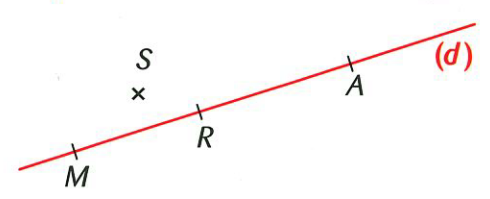
\includegraphics[scale=0.55]{img/droite1}
	\end{center}

	\begin{itemize}
		\item La droite $(d)$ passant par les points $M$ et $R$ se note 
		\item Le point A appartient à la droite $(MR)$, on note :
		\item Le point S n'appartient pas à la droite $(MR)$, on note :
	\end{itemize}
\end{myex}

\begin{mydef}
	Une \kw{demi-droite} est une portion de droite limitée d'un seul côté par un point, son \kw{origine}.
\end{mydef}

\begin{myprop}
	La demi-droite d'origine $A$ et passant par $B$ se note $[AB)$.
\end{myprop}

\begin{myex}
	\begin{center}
		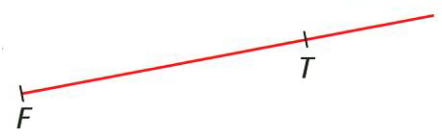
\includegraphics[scale=0.55]{img/demi-droite}
	\end{center}

	La demi droite 
\end{myex}

\begin{mydef}
	Un \kw{segment} est une portion de droite limitée par deux points : ses \kw{extrémités}.
\end{mydef}


\begin{myprop}
	Le segment d'extrémités $A$ et $B$ se note $[AB]$ ou $[BA]$.
\end{myprop}

\begin{myex}
	\begin{center}
		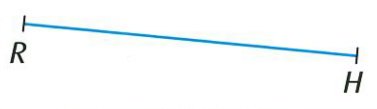
\includegraphics[scale=0.55]{img/segment}
	\end{center}
	
	Le segment 
\end{myex}